%%%%%%%%%%%%%%%%%%%%%%%%%%%%%%%%%%%%%%%%%%%%%%%%%%%%%%%%%%%%
%%% ELIFE ARTICLE TEMPLATE
%%%%%%%%%%%%%%%%%%%%%%%%%%%%%%%%%%%%%%%%%%%%%%%%%%%%%%%%%%%%
%%% PREAMBLE 
\documentclass[9pt,lineno]{elife}
% Use the onehalfspacing option for 1.5 line spacing
% Use the doublespacing option for 2.0 line spacing
% Please note that these options may affect formatting.
% Additionally, the use of the \newcommand function should be limited.


\usepackage{lipsum} % Required to insert dummy text
\usepackage[version=4]{mhchem}
\usepackage{siunitx}
\DeclareSIUnit\Molar{M}

%%%%%%%%%%%%%%%%%%%%%%%%%%%%%%%%%%%%%%%%%%%%%%%%%%%%%%%%%%%%
%%% CUSTOM PACKAGES
%%%%%%%%%%%%%%%%%%%%%%%%%%%%%%%%%%%%%%%%%%%%%%%%%%%%%%%%%%%%

% Required to draw Fig. 1
\usepackage{tikz}
\usetikzlibrary{decorations.pathmorphing}
\usetikzlibrary{shapes.symbols}


% Vim macro to remove color or sout commands:
% 1. place cursor at \ before command
% 2. type "q-d-d-t-{-%-x-ctrl-o-x-q"
% Test:
%\label{pi-silencing}


%%%%%%%%%%%%%%%%%%%%%%%%%%%%%%%%%%%%%%%%%%%%%%%%%%%%%%%%%%%%
%%% ARTICLE SETUP
%%%%%%%%%%%%%%%%%%%%%%%%%%%%%%%%%%%%%%%%%%%%%%%%%%%%%%%%%%%%
\title{Muller's Ratchet in Asexual Populations Doomed to Extinction}

\author[1]{Logan Chipkin}
\author[2,3]{Peter Olofsson}
\author[2]{Ryan C.\ Daileda}
\author[1*]{Ricardo B.\ R.\ Azevedo}
\affil[1]{Department of Biology \& Biochemistry, University of Houston, Houston, Texas, U.S.A.}
\affil[2]{Department of Mathematics, Trinity University, San Antonio, Texas, U.S.A.}
\affil[3]{Department of Mathematics, Physics and Chemical Engineering, Jönköping University, Sweden}


\corr{razevedo@uh.edu}{}
%\corr{email2@example.com}{FS}

%\contrib[\authfn{1}]{These authors contributed equally to this work}
%\contrib[\authfn{2}]{These authors also contributed equally to this work}

%\presentadd[\authfn{1}]{Department, Institute, Country}
%\presentadd[\authfn{4}]{Department, Institute, Country}
% \presentadd[\authfn{5}]{eLife Sciences editorial Office, eLife Sciences, Cambridge, United Kingdom}

%%%%%%%%%%%%%%%%%%%%%%%%%%%%%%%%%%%%%%%%%%%%%%%%%%%%%%%%%%%%
%%% ARTICLE START
%%%%%%%%%%%%%%%%%%%%%%%%%%%%%%%%%%%%%%%%%%%%%%%%%%%%%%%%%%%%

\begin{document}

\maketitle

\begin{abstract}
Please provide an abstract of no more than 150 words. Your abstract should explain the main contributions of your article, and should not contain any material that is not included in the main text.
\end{abstract}


\section{Introduction}

\medskip

\begin{quotation}
``All populations are doomed to eventual extinction.'' \citet{Lynch_MUTATION_1990}
\end{quotation}

In the absence of back mutations, an asexual individual cannot produce offspring carrying fewer deleterious mutations than itself. Indeed, it is always possible that individual offspring will accrue additional deleterious mutations. 
As a result, the class of individuals with the fewest deleterious mutations may, by chance, disappear irreversibly from the population, a phenomenon known as Muller's Ratchet
\citep{Muller_The_1964, Felsenstein_The_1974, Haigh_The_1978}.  Successive ``clicks'' of the Ratchet will cause the fitness of asexual populations to decline.
Muller's Ratchet has been invoked to explain 
the evolution of sex \citep{Muller_The_1964, Felsenstein_The_1974, gor08},
the accelerated rate of evolution of endosymbiotic bacteria \citep{mor96},
and the degeneration of Y-chromosomes \citep{Charlesworth_Model_1978, gor00b}.  

%\red{\sout{The first formal model of Muller's Ratchet assumed a constant population size}} \citep{Haigh_The_1978}, \red{\sout{and this has been standard ever since}} \citep{Gessler_The_1995,Gordo_On_2000,Pamilo_1987}.
%[R: deal with exceptions later. You have to explain the classic model first and then explain why it's not satisfactory.]. 
%\sout{Given that populations subject to the ratchet are expected to decrease in absolute fitness, this assumption is not expected to hold true in general.} 
\citet{Haigh_The_1978} %\red{\sout{'s model emphasized} 
argued that the Ratchet should click at a rate inversely proportional to the size of the least-loaded class in a population.  If $k$ is the lowest number of deleterious mutations present in an individual in the population, 
the size of the least-loaded class at mutation-selection-drift equilibrium is
%
\begin{equation}
  \hat n_k = N e^{-U/s} \quad ,
  \label{eq:haigh}
\end{equation}
%
%\red{[R: this $n_0$ clashes with our notation later.]}
%\red{\sout{as the most important quantity with respect to the rate of the ratchet,}} 
where $N$ is the size of the population, $U$ is the 
expected number of deleterious mutations
per genome per generation, and $s$ is the deleterious effect of a mutation. 
Haigh suggested that genetic drift causes the actual value of $n_k$ to deviate stochastically from $\hat n_k$.  The smaller the value of $\hat n_k$, the greater the probability that $n_k$ will hit zero, causing the Ratchet to click.  
If $\hat n_k > 1$, then after a click of the Ratchet, the size of the new least-loaded class will go to a new equilibrium, $\hat n_{k+1}$, equal to $\hat n_k$ in Equation \ref{eq:haigh}. 
Haigh concluded that Muller's Ratchet should click faster 
in small populations, 
experiencing a high deleterious mutation rate, 
and mutations with milder deleterious effects (low $s$).
Subsequent work has derived more accurate estimates of the rate of clicking of the Ratchet, both when $\hat n_k > 1$ \citep{Stephan_The_1993, gor00b, Gordo_On_2000, met13} and when $\hat n_k < 1$ \citep{Gessler_The_1995, Rouzine_The_2003, Rouzine_The_2008}. 


\begin{figure*}
  \centering
	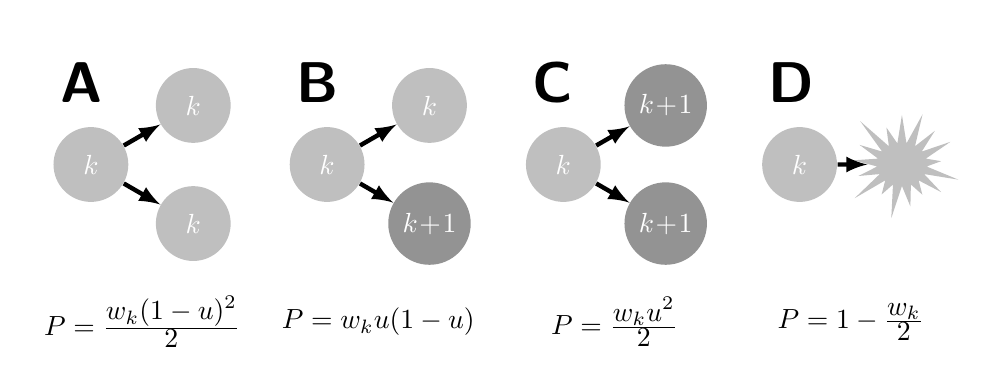
\begin{tikzpicture} 
% Row 1
		\node (par1)       at       (0, 0)       [circle, minimum size=9.5mm, fill=gray!50]      {\textcolor{white}{$k$}};
		\node (off11)      at       (1.3, .75)   [circle, minimum size=9.5mm, fill=gray!50]      {\textcolor{white}{$k$}};
		\node (off12)      at       (1.3, -.75)  [circle, minimum size=9.5mm, fill=gray!50]      {\textcolor{white}{$k$}};
		\draw[-latex, ultra thick]  (par1)  to  (off11);
		\draw[-latex, ultra thick]  (par1)  to  (off12);
		\node (par2)       at       (3, 0)       [circle, minimum size=9.5mm, fill=gray!50]      {\textcolor{white}{$k$}};
		\node (off21)      at       (4.3, .75)   [circle, minimum size=9.5mm, fill=gray!50]      {\textcolor{white}{$k$}};
		\node (off22)      at       (4.3, -.75)  [circle, minimum size=9.5mm,fill=gray!85]      {\textcolor{white}{$k\!+\!1$}};
		\draw[-latex, ultra thick]  (par2)  to  (off21);
		\draw[-latex, ultra thick]  (par2)  to  (off22);
        \node (par3)       at       (6, 0)       [circle, minimum size=9.5mm, fill=gray!50]      {\textcolor{white}{$k$}};
		\node (off31)      at       (7.3, .75)   [circle, minimum size=9.5mm, fill=gray!85]      {\textcolor{white}{$k\!+\!1$}};
		\node (off32)      at       (7.3, -.75)  [circle, minimum size=9.5mm, fill=gray!85]      {\textcolor{white}{$k\!+\!1$}};
		\draw[-latex, ultra thick]  (par3)  to  (off31);
		\draw[-latex, ultra thick]  (par3)  to  (off32);
        \node (ind)        at       (9, 0)       [circle, minimum size=9.5mm, fill=gray!50]      {\textcolor{white}{$k$}};
        \node (dead)       at       (10.3, 0)    [starburst, minimum size=3mm, fill=gray!50]      {\textcolor{gray!50}{$n$}};
        \draw[-latex, ultra thick]  (ind)  to  (dead);
% Row 2
		\node (p1)  at       (0.65, -2)      {$P = \frac{\displaystyle w_k (1-u)^2}{\displaystyle 2}$};
		\node (p2)  at       (3.65, -2)      {$P = w_k u (1-u)$};
        \node (p3)  at       (6.65, -2)      {$P = \frac{\displaystyle w_k u^2}{\displaystyle 2}$};
        \node (p4)  at       (9.65, -2)      {$P = 1-\frac{\displaystyle w_k}{\displaystyle 2}$};
% Labels
\huge
		\node[right] (A)          at       (-.81, 1.04) [circle]  {\sf\textbf{A}};
		\node[right] (B)          at       (2.19, 1.04) [circle]  {\sf\textbf{B}};
		\node[right] (C)          at       (5.19, 1.04) [circle]  {\sf\textbf{C}};
		\node[right] (D)          at       (8.19, 1.04) [circle]  {\sf\textbf{D}};
	\end{tikzpicture}	

 	\caption{Multitype branching process.  At each time step, an individual of type $k$---i.e, with $k$ deleterious mutations (light gray)---can have one of four fates \textbf{(A--D)} with different probabilities, $P$ (see Table \ref{tab:pars}).  
%
It can either die \textbf{(D)}
%
or survive and split into two daughters \textbf{(A--C)}. 
%
The daughters inherit the $k$ mutations from their mother.
%
A daughter can acquire one additional mutation and become a type $k+1$ individual (dark gray) \textbf{(B--C)}.}
	\label{fig:branching}	
\end{figure*}


Beginning with Haigh's foundational study, most research on Muller's Ratchet (including all the papers cited so far) has assumed that population size remains constant as the population accumulates deleterious mutations.  
This assumption is biologically unrealistic---if true, fitness would decline %indefinitely 
continuously but the population would be immortal
%without ever causing the population to go extinct 
\citep{Lynch_MUTATION_1990, mel91}.  Lynch, Gabriel, and colleagues studied more realistic models where the fitness of an individual influences its fertility, and populations experience density-dependent regulation \citep{Lynch_MUTATION_1990, lyn93, Gabriel_MULLER_1993}.  They found that Muller's Ratchet causes population size to decline, which accelerates the Ratchet, which in turn further reduces population size.  This positive feedback results in a ``mutational meltdown'' that drives the population to extinction \citep{Lynch_MUTATION_1990, lyn93, Gabriel_MULLER_1993}.

In one model, \citet{lyn93} considered a population of asexual organisms subject to a carrying capacity of $\widehat N$ individuals.  Each individual produces $R$ offspring.  The number of mutations is Poisson distributed with rate $U$.  The offspring then undergo viability selection with a probability of survival
%
\begin{equation}
  w_k=(1-s)^{k} \quad ,
  \label{eq:fit}
\end{equation}
%
where
$k \geq 0$ is the number of deleterious mutations in the individual offspring,  
and $0 < s < 1$ is the deleterious effect of each mutation. 
If the number of offspring surviving viability selection is $N' > \widehat N$, $N' - \widehat N$ individuals die and $\widehat N$ individuals survive, independently of their fitness; if $N' \leq \widehat N$, all $N'$ individuals survive.  
Reproduction occurs after viability selection and density-dependent regulation.  Assuming that initially all individuals in the population are mutation-free and that $N R > \widehat N$, Muller's Ratchet proceeds in three phases in this model.  
%%%
First, mutations enter the population and accumulate rapidly.  As the distribution of mutation numbers approaches mutation-selection-drift equilibrium mutation accumulation slows down.
%%%
Second, the rate of mutation accumulation settles into a steady rate.  This phase proceeds as in the classic constant population size model of Muller's Ratchet \citep{Haigh_The_1978} and lasts while $N R \, \overline w \gtrsim \widehat N$.
%%%
Third, when mean viability reaches $\overline w = 1/R$ (i.e., when $N R \, \overline w = \widehat N$) the population size begins to decline, triggering mutational meltdown.  During this phase the population is doomed to extinction.


\citet{lyn93} derived some analytical expressions to describe the dynamics of mutation accumulation during the first two phases and the times at which these two phases end.  
However, they did not present any analytical results on the dynamics or duration of the meltdown (third) phase itself.
%%%
Here we model the mutational meltdown phase of Muller's Ratchet using a multi-type branching process.
We derive an analytical approximation for the expected time to extinction under this model
of populations doomed to extinction.  
We find that extinction occurs more quickly in small populations, 
experiencing a high deleterious mutation rate $(u)$, 
and mutations with \emph{more severe} deleterious effects (high $s$).  
Our results differ from predictions on the relationship between the severity of Muller's Ratchet and mutational parameters in populations of constant size.
We also find that mutational meltdown, 
although it does occur in doomed populations,
is not an important determinant of time to extinction. 
Rather, extinction time is approximately inversely proportional to $us$, that is, 
the expected impact of mutations on fitness.

%Thanks for using Overleaf to write your article. Your introduction goes here! Some examples of commonly used commands and features are listed below, to help you get started.

%Here's a second paragraph to test paragraph indents. \lipsum[1]


\section{Model}


\begin{table}[bt]
\caption{\label{tab:pars}Variables and parameters.}
% Use "S" column identifier to align on decimal point 
\begin{tabular}{S l}
\toprule
{Symbol} & Description     \\
\midrule
$u$            & Probability that an individual acquires a deleterious mutation (Figure \ref{fig:branching}).\\
$s$            & Deleterious effect of a mutation (Equation \ref{eq:fit}).\\
$w_k$          & Fitness of an individual of type $k$, i.e.\ with $k$ deleterious mutations (Equation \ref{eq:fit}).\\
%$\varphi_k(x)$ & Probability generating function of the number of $k$-type offspring of a $k$-type individual (Equation \ref{eq:pgf}).\\
$m_{i, j}$     & Expected number of offspring of type $j$ generated by an individual of type $i$ \\
               & (Equation \ref{eq:m}).\\
$n_0$          & Initial number of mutation-free individuals in the population.\\
$n_k$          & Expected number of $k$-type individuals in the population.\\
$N$            & Total population size (Equation \ref{eq:N}).\\
$t_k$          & Expected extinction time of $k$-type individuals in generations, i.e.\ the $k$-th click of the \\
               & Ratchet (Equation \ref{eq:tk}).\\
$\Delta t_k$   & Interval between clicks $k-1$ and $k$ of the Ratchet (Equation \ref{eq:deltat}).\\
$x_k$          & Expected number of $k$-type individuals at the extinction time of type $k-1$ \\
               & (Equation \ref{eq:xk}).\\
$\mathbf{T}$   & Expected extinction time of the entire population in generations (Equation \ref{eq:T}).\\
\bottomrule
\end{tabular}

%\medskip 
%Source: \url{https://www.sedl.org/afterschool/toolkits/science/pdf/ast_sci_data_tables_sample.pdf}

% \tabledata{This is a description of a data source.}

\end{table}

\subsection{Branching process}


A population consists of $N_k$ individuals with $k=0,\, 1,\, 2,\, \ldots$ deleterious mutations.  Below, we refer to individuals with $k$ deleterious mutations as having type $k$.

The size $N = \sum_i N_i$ of the population is allowed to change according to a discrete-time branching process.   
Each generation, an individual of type $k$ reproduces by splitting into two daughters with probability $w_k/2$ and dies with probability $1 - w_k/2$ (Figure \ref{fig:branching}), where $w_k$ is the fitness of an individual of type $k$ (Equation \ref{eq:fit}). 
We assume that all mutations have the same deleterious effect $s$ and do not interact epistatically.  
Fitness is \textit{absolute} in our model.

Any offspring may acquire one deleterious mutation with probability $u$. 
Note that $u$ is defined differently from the mutation rate, $U$, in Haigh's model (Equation \ref{eq:haigh}).
The number of mutant offspring of a surviving individual of any type is binomially distributed  with parameters $2$ and $u$ (Figure \ref{fig:branching}).

This branching process
yields the probability generating function (p.g.f.) of the number of $k$-type offspring of a $k$-type individual 
%
\begin{equation}
  \varphi_{k}(x)=1-\frac{w_k}{2}\left(1-u^2-2u(1\!-\!u)x-(1\!-\!u)^2x^2\right)
  \label{eq:pgf}
\end{equation}
%
and mean reproduction matrix $M$ with entries 
%
\begin{equation}
  \left\{\begin{array}{lll}
            m_{k,k} & = & w_k (1-u)\\
            m_{k,k+1} & = & w_k u\\
            \end{array} \right.
  \label{eq:m}
\end{equation}
%
where $m_{i,j}$ is the expected number of offspring of type $j$ generated by an individual of type $i$.  All other entries of $M$ are 0.

The mean reproduction matrix for generation $t$ is $M^{t}$, the $t$-th power of $M$. For any $t$, all entries of $M^{t}$ below the diagonal are 0. 
Assuming the fitness function in Equation \ref{eq:fit}, we can get an explicit form for the entries $m_{i,j}^{(t)}$ of $M^{t}$:
%
\begin{equation}
  m^{(t)}_{k,k+j} = \displaystyle a^{t-j}b^{j}(1 - s)^{tk\,+\textstyle\frac{j(j-1)}{2}}\prod_{i=1}^{j}\frac{1 - (1 - s)^{t+1-i}}{1 - (1 - s)^{i}}
  \label{eq:mt}
\end{equation}
where $j=0,\,1,\,2,\,\ldots,\; a=m_{0,0}=1-u$, and $b=m_{0,1}=u$.
% 
For a proof, see Appendix 1.  


\begin{figure*}[h!]
\centering
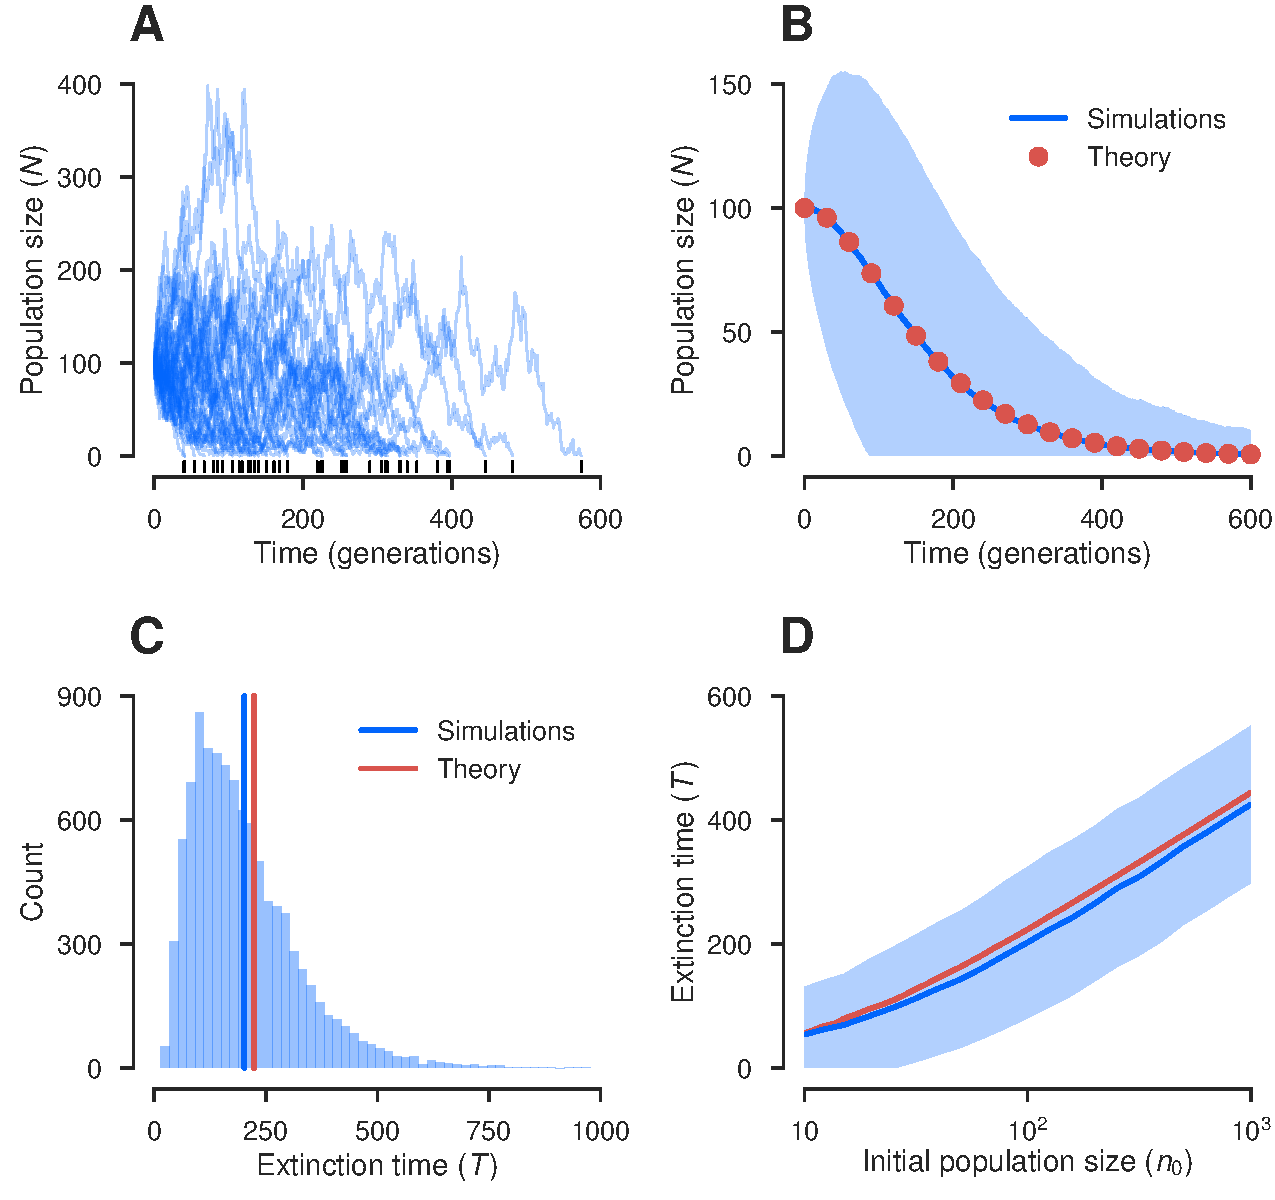
\includegraphics[width=.67\linewidth]{decay.pdf}
\caption{Populations doomed to extinction.  
%
\textbf{(A)} Dynamics of population size, $N$, in 50 populations founded by $n_0=100$ mutation-free individuals and subject to mutations with deleterious effect $s=0.01$ and rate $u=0.01$.  Black vertical lines indicate extinction times.
%
\textbf{(B)} Blue line shows mean $N$ based on stochastic simulations of $10^4$ replicate populations like those shown in \textbf{(A)}.  
Light blue region indicates $\overline{N} \pm 1$ standard deviation (s.d.). If $\mathrm{s.d.} > \overline{N}$, the lower bound of the region was set to zero.  
Red circles indicate expected population size (Equation \ref{eq:N}) every 30 generations.
%
\textbf{(C)} Distribution of extinction times, \textbf{T}, in the stochastic simulations described in \textbf{(B)} (8 replicate populations had $\mathbf{T} > 900$ and are not shown). 
Blue line shows mean \textbf{T} based on the $10^4$ replicate populations.  
Red line shows \textbf{T} calculated numerically (Equation \ref{eq:T}) by assuming that $P(\tau_{k} > 0) = 0$.  
%
\textbf{(D)} Extinction times of populations with the same mutational parameters as those in \textbf{(A)} but with a range of initial populations sizes, $n_0$.
%
Blue line shows mean values of \textbf{T} based on stochastic simulations of $10^4$ replicate populations for 21 values of $n_0$ evenly spaced on a log-scale.
%
Red line shows \textbf{T} calculated numerically.
}
\label{fig:decay}
\end{figure*}


\subsection{Extinction time of individuals of type \emph{k}}


Let $\tau_k$ denote the time of extinction of individuals of type $k$ in a population started from $N_{k}$ ancestors of type $k$ where $N_k$ is a random variable on $\{0,1,2,...\}$ (if $N_k=0$, then $\tau_k=0$).  
There are no individuals of type $i < k$ in the population.
By a standard result from probability theory
%
\begin{equation*}
E[\tau_k]=\sum_{t=0}^{\infty}P(\tau_k>t)
\end{equation*}
%
The time of extinction of the entire type-$k$ subpopulation is the time of extinction of the $N_{k}$ independent subpopulations started from the ancestors. The p.g.f.\ of the number of $k$-type individuals in generation $t$ is given by the $t$-fold composition of $\varphi_k$ (Equation \ref{eq:pgf}) with itself, denoted by $\varphi^{(t)}_k$. We get
%
$$\tau_{k}=\max\{\tau_{k,1},...,\tau_{k,N_{k}}\}$$
%
where $\tau_{k,j}$ is the time of extinction of the subpopulation started from the $j$th individual, $j=1,...,N_k$. If we let $Z_{t}^{(k,j)}$ denote the number of type-$k$ individuals in generation $t$ stemming from the $j$th individual we have the equivalence 
%
\begin{equation*}
\tau_{k,j}\leq n \Leftrightarrow Z_{n}^{(k,j)}=0
\end{equation*}
%
and get the conditional probability given $N_k$
%
\begin{align*}
%
P(\tau_{k}>t|N_k) & =  1-P(\tau_{k}\leq t|N_k)\\[3pt]
           & =  1-\prod_{j=1}^{N_{k}}P(\tau_{k,j}\leq t)\\[3pt]
           & =  1-\left(\varphi_{k}^{(t)}(0)\right)^{N_{k}}
\end{align*}
%
for $t>0$ which gives 
%
\begin{equation*}
%
E[\tau_{k}] = P(\tau_{k}>0) + E\left[\sum_{t=1}^{\infty}\left(1-\left(\varphi_{k}^{(t)}(0)\right)^{N_{k}}\right)\right]
%
%\label{expected1}
\end{equation*}
%
With $n_k=E[N_k]$, a first-order Taylor approximation gives 
%
\begin{equation}
%
E[\tau_{k}] \approx P(\tau_{k}>0) + \sum_{t=1}^{\infty}\left(1-\left(\varphi_{k}^{(t)}(0)\right)^{n_{k}}\right)
%
\label{eq:tauk}
\end{equation}
%
Note that for $k=0$ we have $P(\tau_{0}>0)=1$ because there are always individuals present at time $0$. For $k>0$, however, we have $P(\tau_{k}>0)<1$ because, for example, 
the entire population may already be extinct
%type 1 
in generation 1. 

In a similar way, we get the variance as
%
$$\mbox{Var}[\tau_{k}]=E[\tau_{k}(\tau_{k}-1)]+E[\tau_{k}]-E^{2}[\tau_{k}]$$
%
where
%
\begin{align*}
%
E[\tau_{k}(\tau_{k}-1)] & =  2\sum_{t=1}^{\infty}tP(\tau_{k}>t)\\[5pt]
& \approx  2\sum_{t=1}^{\infty}t\left(1-\left(\varphi_{k}^{(t)}(0)\right)^{n_k}\right)
%
\end{align*}


\begin{figure*}[h!]
\centering
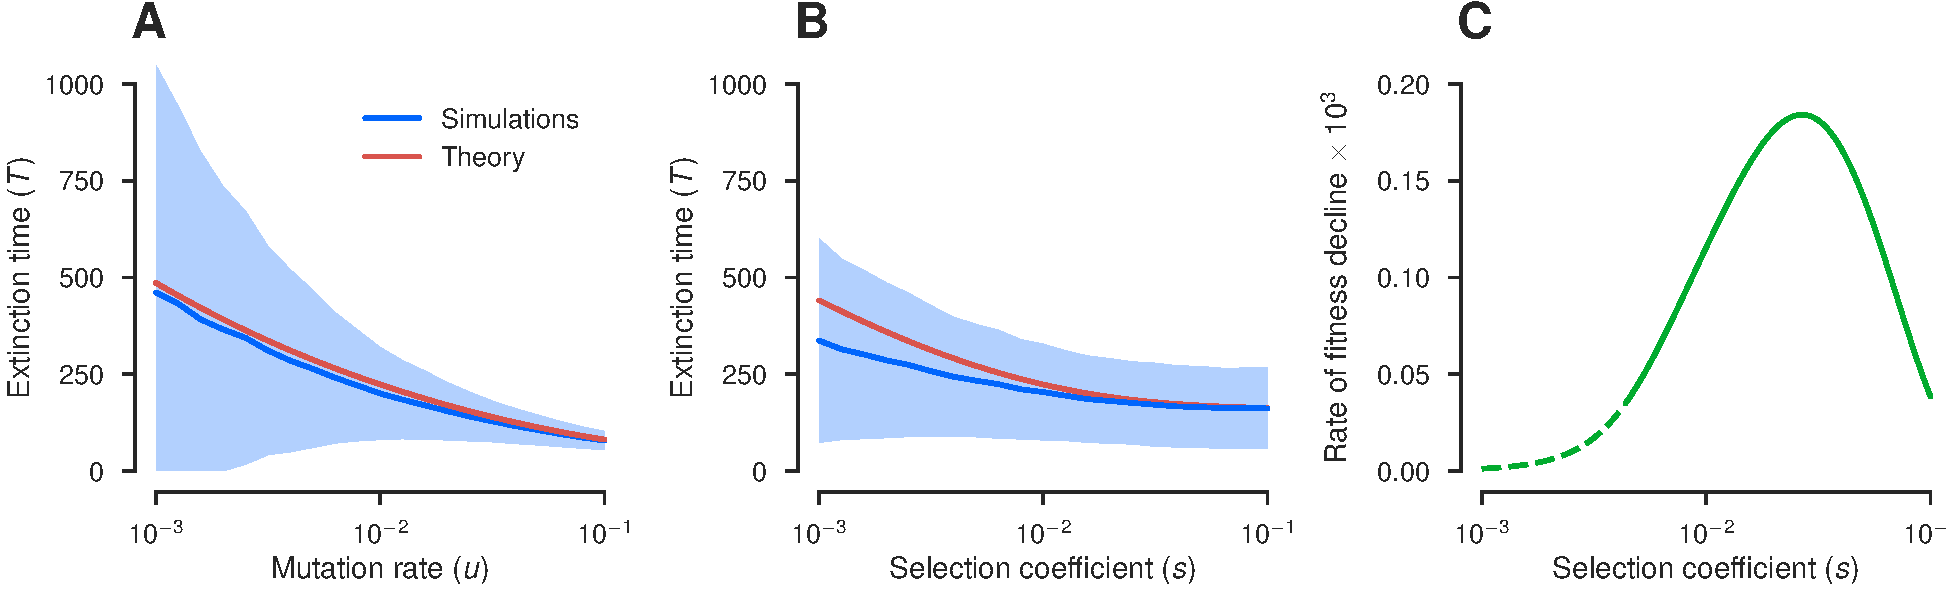
\includegraphics[width=\linewidth]{valid.pdf}
\caption{
Mutational parameters have different effects on extinction time in doomed populations and Muller's Ratchet in populations of constant size.
%
\textbf{(A--B)} Values are expected extinction times, \textbf{T}, in populations founded by $n_0=100$ mutation-free individuals but with different mutational parameters.
%
\textbf{(A)} Mutations have deleterious effect $s=0.01$ and a range of mutation rates, $u$.
%
\textbf{(B)} Mutations have rate $u=0.01$ and a range of deleterious effects, $s$.
%
Red lines show \textbf{T} calculated numerically (Equation \ref{eq:T}) by assuming that $P(\tau_{k} > 0) = 0$ for 41 values of the parameter being manipulated, evenly spaced on a log-scale.
%
Blue lines show mean values of \textbf{T} based on stochastic simulations of $10^4$ replicate populations for 21 values of the parameter being manipulated, evenly spaced on a log-scale.
%
Light blue regions indicate $\overline{\mathbf{T}} \pm 1\, \mathrm{s.d.}$  If $\mathrm{s.d.} > \overline{\mathbf{T}}$, the lower bound of the region was set to zero.
%
\textbf{(C)} Severity of Muller's Ratchet in populations of constant size and a deleterious mutation rate of $U = 0.01$ per genome per generation.  Values are the expected declines in mean fitness per thousand generations, $10^3 \times s/\Delta t$, for 101 values of $s$ evenly spaced on a log-scale.  
$\Delta t$ is the time between clicks of the Ratchet calculated using the method of \citet{gor00b, Gordo_On_2000}.
Dashed and solid lines indicate $\hat n_k < 10$ and $\hat n_k \geq 10$, respectively (Equation \ref{eq:haigh}).  
%
The trend shown in \textbf{(C)} was confirmed by simulation (not shown).
}
\label{fig:valid}
\end{figure*}


\subsection{Extinction time of the entire population}


By well-known results from the theory of branching processes, the extinction time of the entire population has finite mean only in the {\em subcritical} case, that is, when the mean number of offspring per individual is less than 1. 
%Let $R_k$ be 
The expected number of offspring of type $k$ produced by an individual of type $k$ is $m_{k,k}$ (Equation \ref{eq:m}).  
%in the next time step so that $$R_k = 2p(1-u)w_k$$
If $m_{k,k}=1$ (the \emph{critical} case), the extinction time $\tau_k$ is finite but has an infinite mean and if $m_{k,k} > 1$ (the {\em supercritical} case), $\tau_k$ itself may assume the value $\infty$.  

Equation \ref{eq:m} shows that $m_{k,k} < 1$ (the {\em subcritical} case) for individuals of any type $k$ provided all mutations are deleterious $(0<s<1)$ and the mutation rate is nonzero $(u>0)$.  Thus, the expected extinction time of every type $k$ is finite.  
In other words, the population is ``doomed to eventual extinction'' \citep{Lynch_MUTATION_1990}.  

Start with a fixed number $n_{0}$ of mutation-free individuals and denote by $T_{0}$ the time (generation) of extinction of this class. Conditioned on $T_{0}$, the expected number of individuals in class 1 (those with $k=1$ mutation) is therefore 
%
\begin{equation}
m_{0,1}^{(T_0)}
\label{eq:mT0}
\end{equation}
%
(see Equation \ref{eq:mt})
which we note is a function of the random variable $T_{0}$. Thus, the expected number of individuals in class 1 at the time of extinction of class 0 is obtained by taking the expected value in Equation \ref{eq:mT0}. To this end, recall Equation \ref{eq:mt} and define the function 
%
\begin{equation*}
g_1(\cdot)=m_{0,1}^{(\cdot)}
%\label{g1defined}
\end{equation*}
%
so that 
%
\begin{align*}
%
E\left[m_{0,1}^{(T_{0})}\right] &=  E[g_{1}(T_{0})]\\
&\approx  g_{1}\left(E[T_{0}]\right)
%
\end{align*}
%
where we use a first-order Taylor approximation. To generalize the idea, 
% let $a=2p(1-u)$ and $b=2pu$ as before, and 
we define the 
expected number of descendants of type $j$ from a mutation-free individual after $t$ generations
%
\begin{equation}
g_{j}(t) = \left\{\begin{array}{lll}
%
    0              & , & t<j       \\ [4pt]
	m^{(t)}_{0, j} & , & t \geq j
    \end{array}
%
\right. 
\label{eq:gj}
\end{equation}
%
(see Equation \ref{eq:mt}).

\begin{figure*}[h!]
\centering
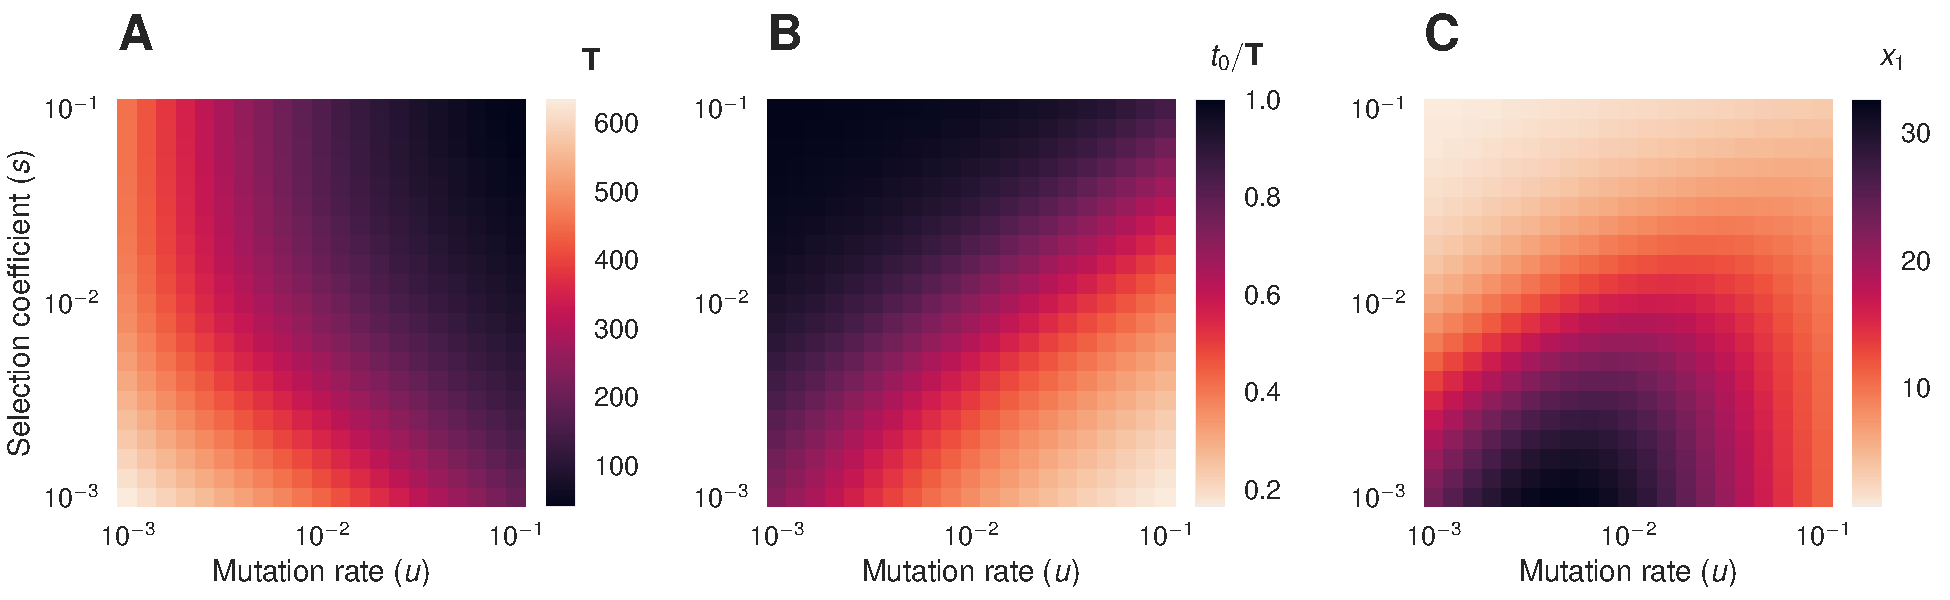
\includegraphics[width=\linewidth]{heat.pdf}
\caption{High mutation rate and mutations of large effect accelerate extinction in doomed populations.  
%
\textbf{(A)} Expected extinction time, $\mathbf{T}$, of populations founded by $n_0=100$ mutation-free individuals and subject to mutations with deleterious effect $s$ and rate $u$.  \textbf{T} was calculated numerically (Equation \ref{eq:T}) by assuming that $P(\tau_{k} > 0) = 0$ for $21\times21=441$ combinations of values of $s$ and $u$ evenly spaced on a log-scale.
%
\textbf{(B)} Expected extinction time of the mutation-free class, $t_0$ (Equation \ref{eq:t0}), as a proportion of \textbf{T} for the populations shown in \textbf{(A)}. 
%
\textbf{(C)} Expected number of individuals with $k=1$ mutation at $t_0$, $x_1$ (Equation \ref{eq:xk}), for the populations shown in \textbf{(A)}.
}
\label{fig:heat}
\end{figure*}

Now let $T_{k}$ be the extinction time for type $k$ and let $t_{k}=E[T_{k}]$. Then we have the approximation
%
\begin{equation}
E\left[m_{0,k+j}^{(T_{k})}\right]\approx g_{k+j}(t_{k})
\label{eq:approx}
\end{equation}
%
the expected number of individuals of type $k+j$ at the extinction of type $k$ for $j=1,2,\ldots$ The expected extinction time of the entire population is
%
\begin{equation}
%
\mathbf{T} = \lim_{k\rightarrow\infty}t_{k} \quad .
%
\label{eq:T}
\end{equation}
%
Now let $X_{T_{k-1}}^{(k)}$ 
be the number of $k$-type individuals at the extinction time of type $k-1$ and let 
%
\begin{equation}
%
x_{k} = E\left[X_{T_{k-1}}^{(k)}\right] \approx n_{0} \, g_{k}(t_{k-1}) \quad .
%
\label{eq:xk}
\end{equation}
%
From Equation \ref{eq:tauk}, the expected extinction times of consecutive classes can be computed as 
%
\begin{equation}
%
t_{k}\approx t_{k-1}+P(\tau_{k}>0)+\sum_{t=1}^{\infty}\left(1-\left(\varphi_{k}^{(t)}(0)\right)^{x_{k}}\right)
%
\label{eq:tk}
\end{equation}
%
where $n_0$ is the initial population size.  
Note that $t_k$ is the time of the $k$-th click of the Ratchet.
As we noted above, for $k=0$ we have $P(\tau_{0}>0)=1$ 
(Equation \ref{eq:tauk}).  Thus, if the population is founded by $n_0$ mutation-free individuals, the time to extinction of the mutation-free class is given exactly by
%
\begin{equation}
t_{0} = 1+\sum_{t=1}^{\infty}\left(1-\left(\varphi_{k}^{(t)}(0)\right)^{n_{0}}\right) \quad .
\label{eq:t0}
\end{equation}
%
When $k>0$, Equation \ref{eq:tk} is an approximation for two reasons.  
First, because $x_k$ is approximate (Equation \ref{eq:xk}).
Second, because type $k$ may be extinct already at the time $T_{k-1}$ when type $k-1$ goes extinct and, therefore, $P(\tau_{k}>0)<1$.
We can place bounds on $P(\tau_{k}>0)$ by noting that
%
\begin{equation}
\tau_{k} > 0 \Leftrightarrow X_{T_{k-1}}^{(k)} > 0
\label{eq:tauk2}
\end{equation}
%
and that if $Y$ is any random variable on $\{0, 1, 2, ...\}$ we have
%
\begin{align}
%
E[Y]  & =   E\left[Y|Y>0\right] P(Y>0)\nonumber\\
      & \geq  P(Y>0)
%
\label{eq:exp}
\end{align}
%
By Equations \ref{eq:xk}, \ref{eq:tauk2}, and \ref{eq:exp} we get the bounds 
%
\begin{equation}
%
0 \leq P(\tau_{k} > 0) \leq \min(1,x_{k}) \quad .
\label{eq:Pbounds}
%
\end{equation}
Because extinction of the whole population is irreversible, $P(\tau_{k} > 0)$ is expected to decline for successive classes:
\begin{equation*}
P(\tau_k>0) \leq P(\tau_{k-1}>0) \quad .
\end{equation*}
%
We calculate \textbf{T} numerically (Equation \ref{eq:T}) by assuming that $P(\tau_{k} > 0) = 0$ and computing Equation \ref{eq:tk} until the following criterion is met 
\begin{equation*}
t_k - t_{k-1} < 10^{-6} \quad .
\end{equation*}


\subsection{Large initial population size}


The expected time to extinction of the mutation-free class, $t_0$, is given by Equation \ref{eq:t0}.
%Motivated by the behavior of $t_0$ as a function of $n_0$, we next turn to investigating the effect of large initial population size on extinction time. Specifically, we investigate the asymptotic behavior of $t_{0}$ as $n_{0}$ approaches infinity. 
Following \citet{Jagers_On_2007}, there exists a sequence $c(n_0)\to c$ as $n_0\to\infty$ such that
%
\begin{equation}
t_0 = -\frac{\ln n_0 + c(n_0)}{\ln m_{0,0}} \quad ,
\label{eq:jagers}
\end{equation}
%
where $m_{0,0} = 1-u <1$ is the expected number of mutation-free offspring per mutation-free individual and $n_0$ is the initial number of mutation-free individuals.  Note that the value of $c$ depends on $u$ (e.g., for $u=0.01$ and 0.02, numerical estimates using Equations \ref{eq:t0} and \ref{eq:jagers} yield $c=3.3737$ and 2.7058, respectively).

Equation \ref{eq:jagers} shows that $t_0$ grows logarithmically with $n_0$ 
with a slope of $-1/\ln m_{0,0}$.  If $u$ is small, the slope is approximately $1/u$.  Thus, increasing initial population size delays extinction of the mutation-free class more when the mutation rate is low than when it is high.

The value of $t_0$ is not affected by the effects of mutations, $s$ (Equations \ref{eq:t0} and \ref{eq:jagers}), because the rate at which individuals ``leave'' the mutation-free class is independent of $s$.  The selection coefficient does, however, affect the size of the new least-loaded class (i.e., individuals with $k=1$ mutation), $x_1$ (Equation \ref{eq:xk}), and therefore the total time to extinction. 

We now investigate the limiting behavior of $x_1$ as $n_0\to\infty$. By Equations \ref{eq:xk} and \ref{eq:jagers} we get 
%
\begin{align}
%
x_{1} &\approx n_0 \, g_{1}(t_0) \nonumber \\[3pt]
%      &= \frac{n_0 \, u}{s} \, (1-u)^{t_0-1} \left(1-(1-s)^{t_0}\right) \nonumber \\[3pt]
      &= \frac{C(n_0) u}{s(1-u)} \left(1-(1-s)^{t_0}\right) \nonumber \\[3pt]
      &\to \frac{C u}{s(1-u)}
%
\label{eq:x1}
\end{align}
%
as $n_0\to\infty$, where $C(n_0) = e^{c(n_0)}$. If $u$ is small and $n_0$ is large, 
Equation \ref{eq:x1} becomes $x_1 \approx C u / s$.
Interestingly, Equation \ref{eq:x1} shows that $x_1$ approaches a constant as $n_0$ increases.

\subsection*{Change in population size}


If a population is founded by $n_0$ mutation-free individuals, the expected total population size $t$ generations later is
%
\begin{equation}
E\left[N(t)\right] = n_0 \sum_{j=0}^t{g_{j}(t)}      
\label{eq:N} %\nonumber\\[2pt]
%
%&=n_0 \prod_{j=0}^t\left(1 + u \sum_{i=1}^{j-1}\binom{j-1}{i}(-s)^{i}\right) \\
%&=n_0 \prod_{j=0}^t\left(1-\frac{u \left(1-s-(1-s)^j\right)}{1-s}\right) \\
%
%&\approx n_0 - n_0 u s \binom{t}{2} 
%\label{eq:Napprox}
\end{equation}
%
(see Equation \ref{eq:gj}).
%Equation \ref{eq:Napprox} is exact for $t \leq 2$ and is a first-order Taylor expansion around $s=0$ for $t > 2$.
%

Initially, $N(0) = n_0$.  Since all individuals have the same fitness, the population size is not expected to change in the following generation: $E\left[N(1)\right] = n_0$.  One generation later, the population size is expected to decline by $E\left[N(2)\right] - E\left[N(1)\right] = - n_0us$.  In subsequent generations, if mutations have small effects, the population size is expected to continue to decline at approximately the same rate
%Using Equation \ref{eq:N}, the expected change in population size from one generation to the next is approximately
%
\begin{equation}
E\left[N(t+1)\right] - E\left[N(t)\right] \approx -n_0 u s t \quad 
\label{eq:deltaN}
\end{equation}



\begin{figure*}[h!]
\centering
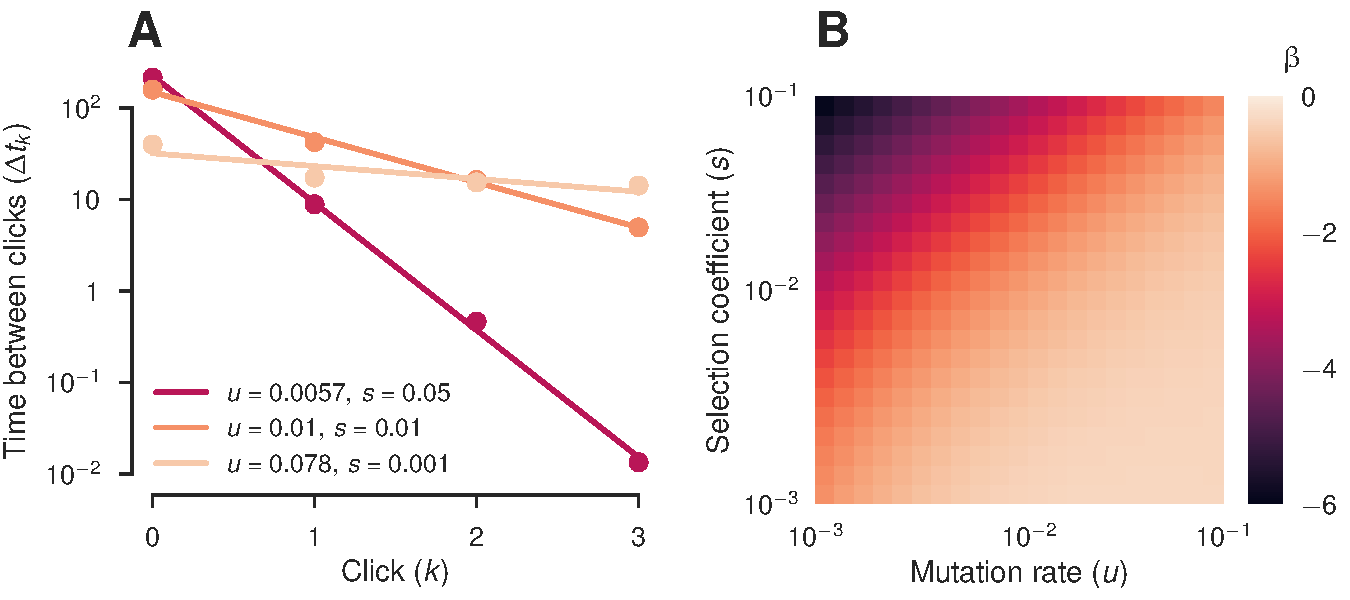
\includegraphics[width=.71\linewidth]{melt.pdf}
\caption{Mutational meltdown does not explain extinction time in doomed populations.  
%
\textbf{(A)} Circles denote time between clicks, $\Delta t_k$ (Equation \ref{eq:deltat}).  Click $k$ indicates the extinction of $k$-type individuals.  Values of $t_0$ were calculated using Equation \ref{eq:tk}; values of $t_1, t_2,$ and $t_3$ were calculated using Equation \ref{eq:tk} by assuming that $P(\tau_{k} > 0) = 0$.
Note that $\Delta t_k$ is displayed on a log-scale.  Each combination of mutational parameters results in populations having the same expected extinction time $(\mathbf{T} = 223.52)$.  Lines indicate linear regression fits (meltdown rates: $\beta = -3.20, -1.14$ and $-0.32$, respectively).
%
\textbf{(B)} Meltdown rates, $\beta$, calculated as shown in \textbf{(A)} for $21\times21=441$ combinations of values of $s$ and $u$ evenly spaced on a log-scale.
}
\label{fig:melt}
\end{figure*}














\section{Results (Level 1 heading)}


\subsection{Level 2 Heading}

\lipsum[3]

\subsubsection{Level 3 Heading}

\lipsum[5]

\paragraph{Level 4 Heading}
\lipsum[7]

\section{Discussion}

\lipsum[9]

\section{Methods and Materials}

Guidelines can be included for standard research article sections, such as this one. 

\lipsum[3]

\section{Some \LaTeX{} Examples}
\label{sec:examples}

Use section and subsection commands to organize your document. \LaTeX{} handles all the formatting and numbering automatically. Use ref and label commands for cross-references.

\subsection{Figures and Tables}

Use the table and tabular commands for basic tables --- see \TABLE{example}, for example. 

You can upload a figure (JPEG, PNG or PDF) using the project menu. To include it in your document, use the \verb|\includegraphics| command as in the code for \FIG{view}. 

For a half-width figure or table with text wrapping around it, use 

\begin{verbatim}
\begin{wrapfigure}{l}{.46\textwidth}
  \includegraphics[width=\hsize]{...}
  \caption{...}\label{...}
\end{wrapfigure}
\end{verbatim}
%
as in \FIG{halfwidth}. For tables:

\begin{verbatim}
\begin{wraptable}{l}{.46\textwidth}{
  \begin{tabular}{...}
  ...
  \end{tabular}}
  \caption{...}\label{...}
\end{wraptable}
\end{verbatim}

Be careful with these, though, as they may behave strangely near page boundaries, sectional headings, or in the neighbourhood of lists or too many floats.

Labels for main videos can be added with \verb|\video| e.g.

\video{Ths is a description of a main video.}\label{video:mv1}
\video{Another!}

Labels for video supplements can be added within \texttt{figure} environments, after the \texttt{caption}, using the \verb|\videosupp| command: see \VIDEOSUPP[view]{sv1} for an example.

If you use the following prefixes for your \verb|\label|:
%
\begin{description}
\item[Figures] \texttt{fig:}, e.g.~\verb|\label{fig:view}|
\item[Figure Supplements] \texttt{figsupp:}, e.g.~\verb|\label{figsupp:sf1}|\\
(we'll assume \texttt{figsupp:sf1} is a figure supplement of \texttt{fig:view} in our example)
\item[Figure source data] \texttt{figdata:}, e.g.~\verb|\label{figdata:first}|
\item[Videos] \texttt{video:}, e.g.~\verb|\label{video:mv1}|
\item[Video supplements] \texttt{videosupp:}, e.g.~\verb|\label{videosupp:sv1}|
\item[Tables] \texttt{tab:}, e.g.~\verb|\label{tab:example}|
\item[Equations] \texttt{eq:}, e.g.~\verb|\label{eq:CLT}|
\item[Boxes] \texttt{box:}, e.g.~\verb|\label{box:simple}|
\end{description}
%
you can then use the convenience commands \verb|\FIG{view}|, \verb|\FIGSUPP[view]{sf1}|, \verb|\TABLE{example}|, \verb|\EQ{CLT}|, \verb|\BOX{simple}|, \verb|\FIGDATA[view]{first}|, \verb|\VIDEO{mv1}| and \verb|{\VIDEOSUPP}[view]{sv1}| \emph{without} the label prefixes, to generate cross-references \FIG{view}, \FIGSUPP[view]{sf1},  \TABLE{example}, \EQ{CLT}, \BOX{simple}, \FIGDATA[view]{first}, \VIDEO{mv1} and \VIDEOSUPP[view]{sv1}. Alternatively, use \verb|\autoref| with the full label, e.g.~\autoref{first:app} (although this may not work correctly for figures and tables in the appendices or boxes nor supplements at present).

Really wide figures or tables, that take up the entire page, including the gutter space: use \verb|\begin{fullwidth}...\end{fullwidth}| as in \FIG{fullwidth}. And sometimes you may want to use feature boxes like \BOX{simple}.

\begin{wrapfigure}{l}{.46\textwidth}
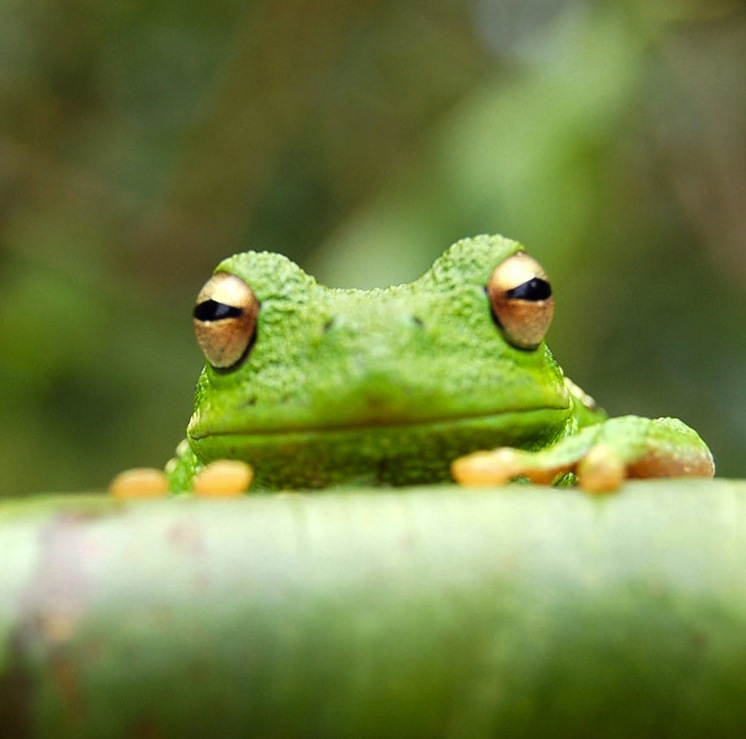
\includegraphics[width=\hsize]{frog}
\caption{A half-columnwidth image using wrapfigure, to be used sparingly. Note that using a wrapfigure before a sectional heading, near other floats or page boundaries is not recommended, as it may cause interesting layout issues. Use the optional argument to wrapfigure to control how many lines of text should be set half-width alongside it.}
\label{fig:halfwidth}
\end{wrapfigure}

Some filler text to sit alongside the half-width figure. \lipsum[1-2]

\begin{figure}
\begin{fullwidth}
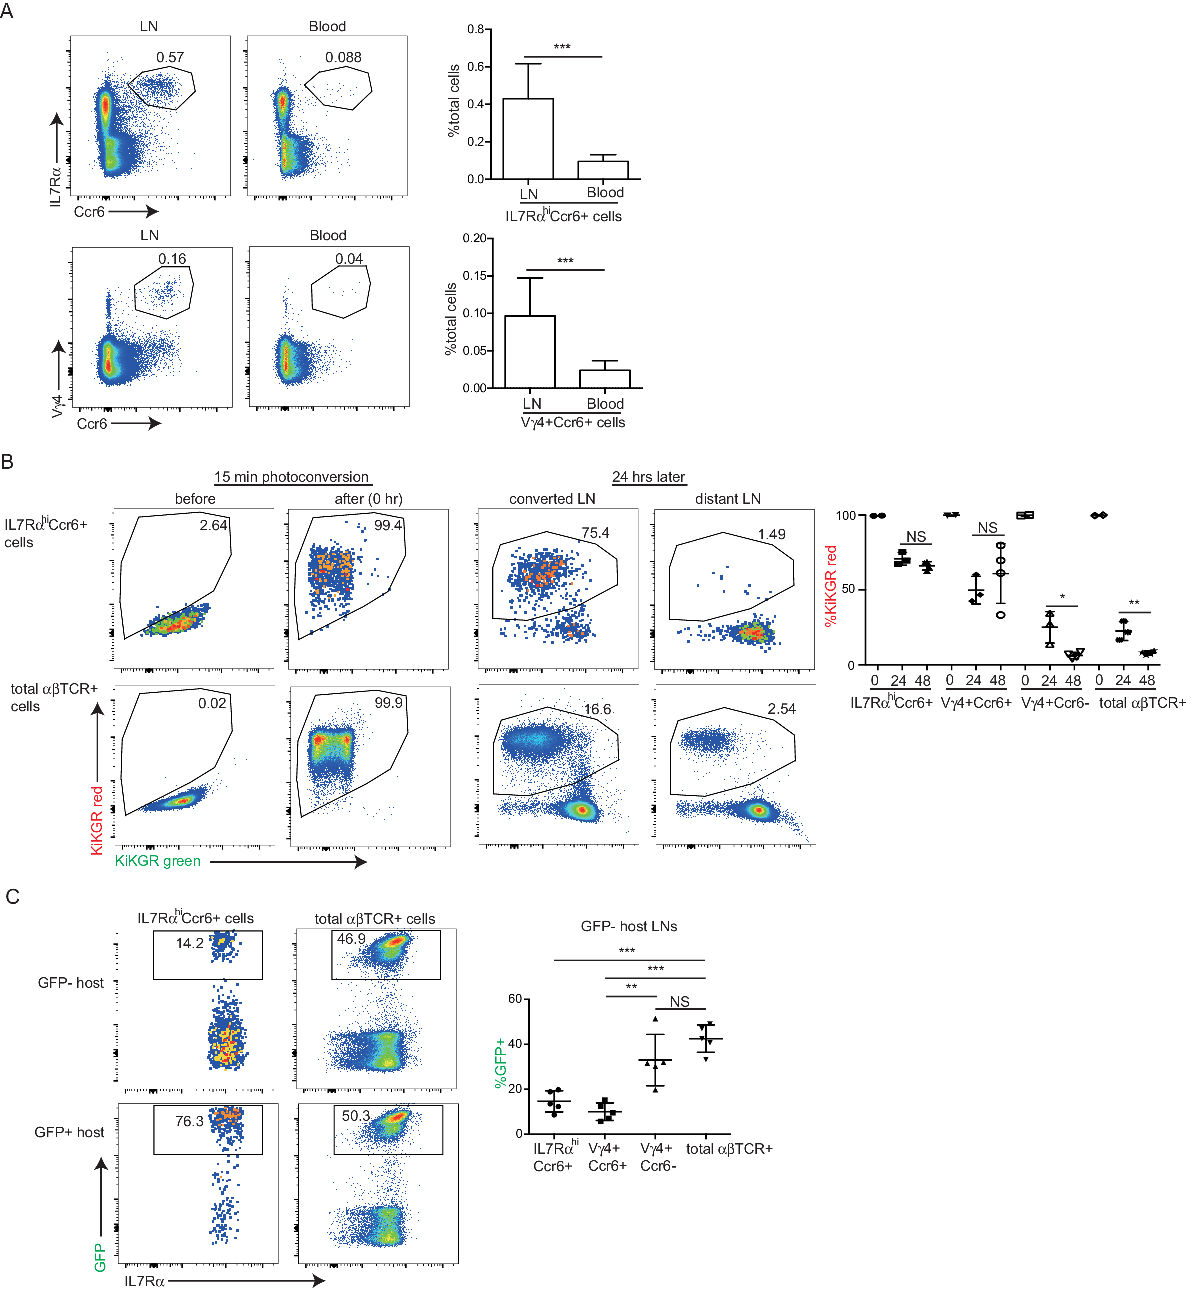
\includegraphics[width=0.95\linewidth]{elife-18156-fig2}
\caption{A very wide figure that takes up the entire page, including the gutter space.}
\label{fig:fullwidth}
\figsupp{There is no limit on the number of Figure Supplements for any one primary figure. Each figure supplement should be clearly labelled, Figure 1--Figure Supplement 1, Figure 1--Figure Supplement 2, Figure 2--Figure Supplement 1 and so on, and have a short title (and optional legend). Figure Supplements should be referred to in the legend of the associated primary figure, and should also be listed at the end of the article text file.}{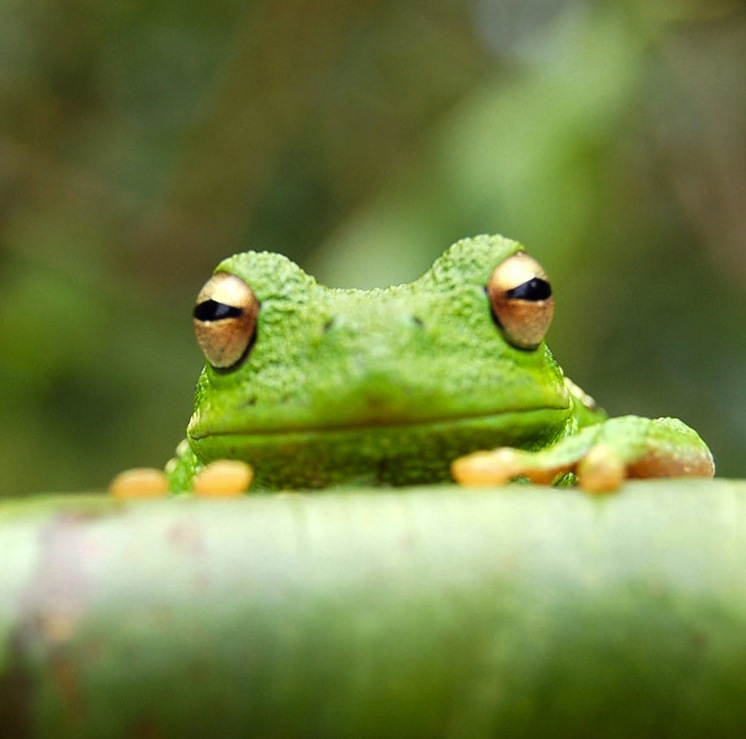
\includegraphics[width=5cm]{frog}}
\end{fullwidth}
\end{figure}

\subsection{Citations}

LaTeX formats citations and references automatically using the bibliography records in your .bib file, which you can edit via the project menu. Use the \verb|\cite| command for an inline citation, like \cite{Aivazian917}, and the \verb|\citep| command for a citation in parentheses \citep{Aivazian917}. The LaTeX template uses a slightly-modified Vancouver bibliography style. If your manuscript is accepted, the eLife production team will re-format the references into the final published form. \emph{It is not necessary to attempt to format the reference list yourself to mirror the final published form.} Please also remember to \textbf{delete the line} \verb|\nocite{*}| in the template just before \verb|\bibliography{...}|; otherwise \emph{all} entries from your .bib file will be listed! 

\begin{featurebox}
\caption{This is an example feature box}
\label{box:simple}
This is a feature box. It floats!
\medskip

\includegraphics[width=5cm]{example-image}
\featurefig{`Figure' and `table' captions in feature boxes should be entered with \texttt{\textbackslash featurefig} and \texttt{\textbackslash featuretable}. They're not really floats.}

\lipsum[1]
\end{featurebox}

\subsection{Mathematics}

\LaTeX{} is great at typesetting mathematics. Let $X_1, X_2, \ldots, X_n$ be a sequence of independent and identically distributed random variables with $\text{E}[X_i] = \mu$ and $\text{Var}[X_i] = \sigma^2 < \infty$, and let
\begin{equation}
\label{eq:CLT}
S_n = \frac{X_1 + X_2 + \cdots + X_n}{n}
      = \frac{1}{n}\sum_{i}^{n} X_i
\end{equation}
denote their mean. Then as $n$ approaches infinity, the random variables $\sqrt{n}(S_n - \mu)$ converge in distribution to a normal $\mathcal{N}(0, \sigma^2)$.

\lipsum[3] 

\begin{figure}
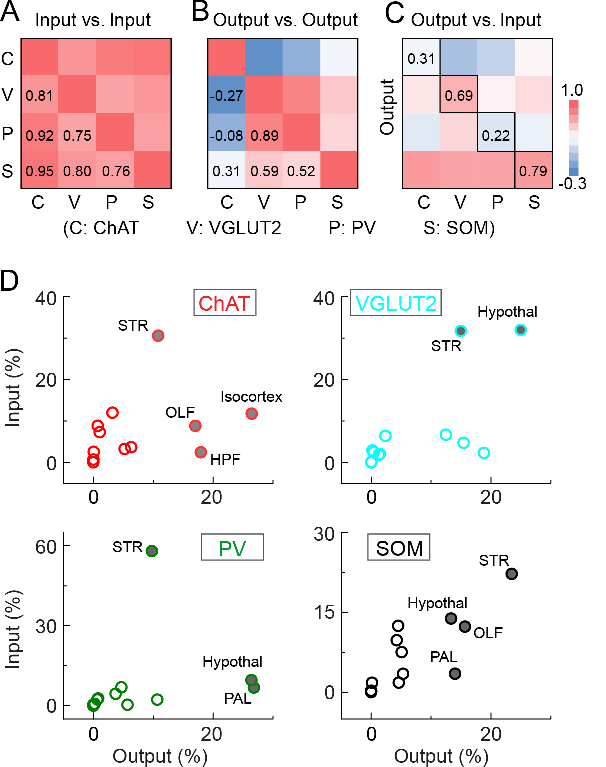
\includegraphics[width=\linewidth]{elife-13214-fig7}
\caption{A text-width example.}
\label{fig:view}
%% If the optional argument in the square brackets is "none", then the caption *will not appear in the main figure at all* and only the full caption will appear under the supplementary figure at the end of the manuscript.
\figsupp[Shorter caption for main text.]{This is a supplementary figure's full caption, which will be used at the end of the manuscript.}{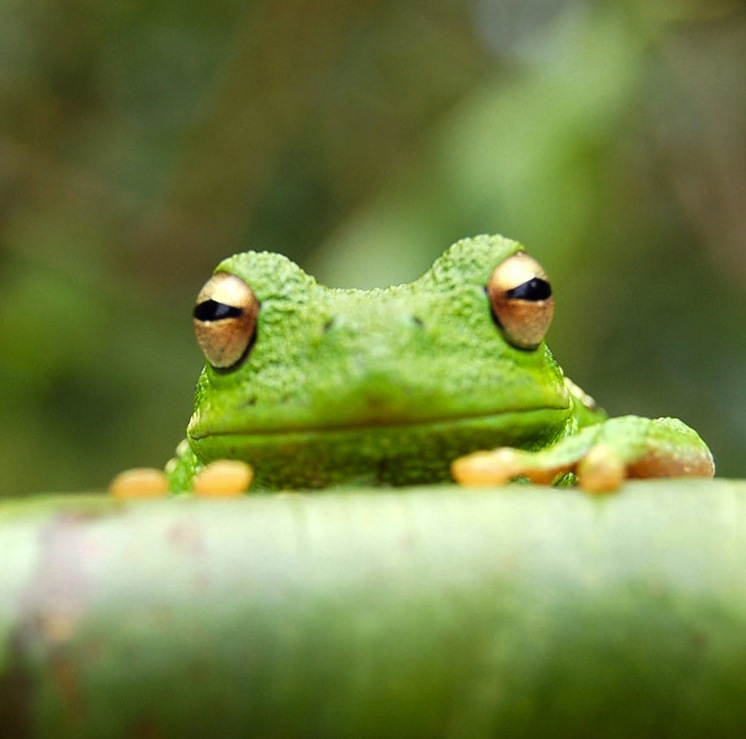
\includegraphics[width=6cm]{frog}}\label{figsupp:sf1}
\figsupp{This is another supplementary figure.}{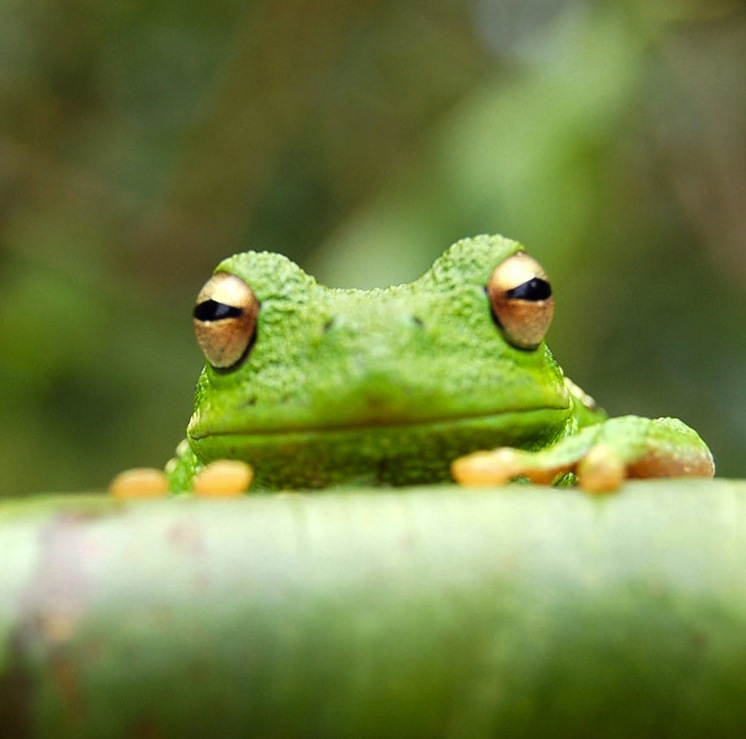
\includegraphics[width=6cm]{frog}}
\videosupp{This is a description of a video supplement.}\label{videosupp:sv1}
\figdata{This is a description of a data source.}\label{figdata:first}
\figdata{This is another description of a data source.}\label{figdata:second}
\end{figure}

\subsection{Other Chemistry Niceties}

You can use commands from the \texttt{mhchem} and \texttt{siunitx} packages. For example: \ce{C32H64NO7S}; \SI{5}{\micro\metre}; \SI{30}{\degreeCelsius}; \SI{5e-17}{\Molar}

\subsection{Lists}

You can make lists with automatic numbering \dots

\begin{enumerate}
\item Like this,
\item and like this.
\end{enumerate}
\dots or bullet points \dots
\begin{itemize} 
\item Like this,
\item and like this.
\end{itemize}
\dots or with words and descriptions \dots
\begin{description}
\item[Word] Definition
\item[Concept] Explanation
\item[Idea] Text
\end{description}

Some filler text, because empty templates look really poorly. \lipsum[1]


\section{Acknowledgments}

Additional information can be given in the template, such as to not include funder information in the acknowledgments section.

\nocite{*} % This command displays all refs in the bib file. PLEASE DELETE IT BEFORE YOU SUBMIT YOUR MANUSCRIPT!
\bibliography{bibliography}

%%%%%%%%%%%%%%%%%%%%%%%%%%%%%%%%%%%%%%%%%%%%%%%%%%%%%%%%%%%%
%%% APPENDICES
%%%%%%%%%%%%%%%%%%%%%%%%%%%%%%%%%%%%%%%%%%%%%%%%%%%%%%%%%%%%

\appendix
\begin{appendixbox}
\label{first:app}
\section{Firstly}
\lipsum[1]

%% Sadly, we can't use floats in the appendix boxes. So they don't "float", but use \captionof{figure}{...} and \captionof{table}{...} to get them properly caption.
\begin{center}
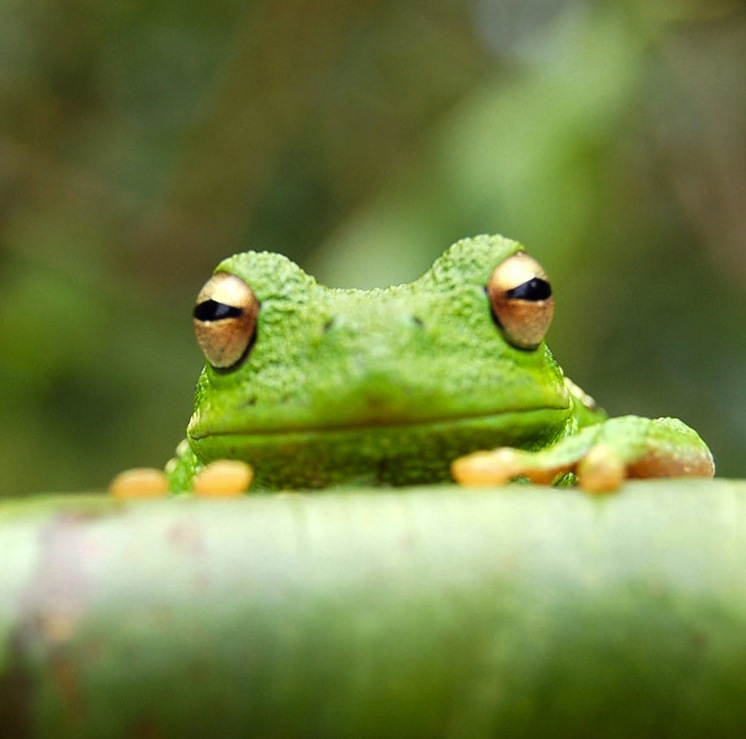
\includegraphics[width=\linewidth,height=7cm]{frog}
\captionof{figure}{This is a figure in the appendix}
\end{center}

\section{Secondly}

\lipsum[5-8]

\begin{center}
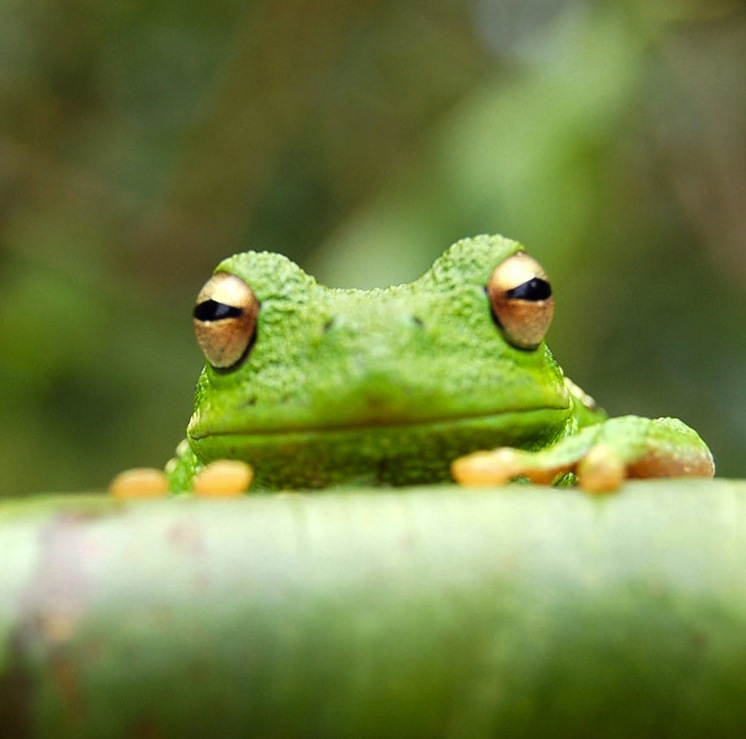
\includegraphics[width=\linewidth,height=7cm]{frog}
\captionof{figure}{This is a figure in the appendix}
\end{center}

\end{appendixbox}

\begin{appendixbox}
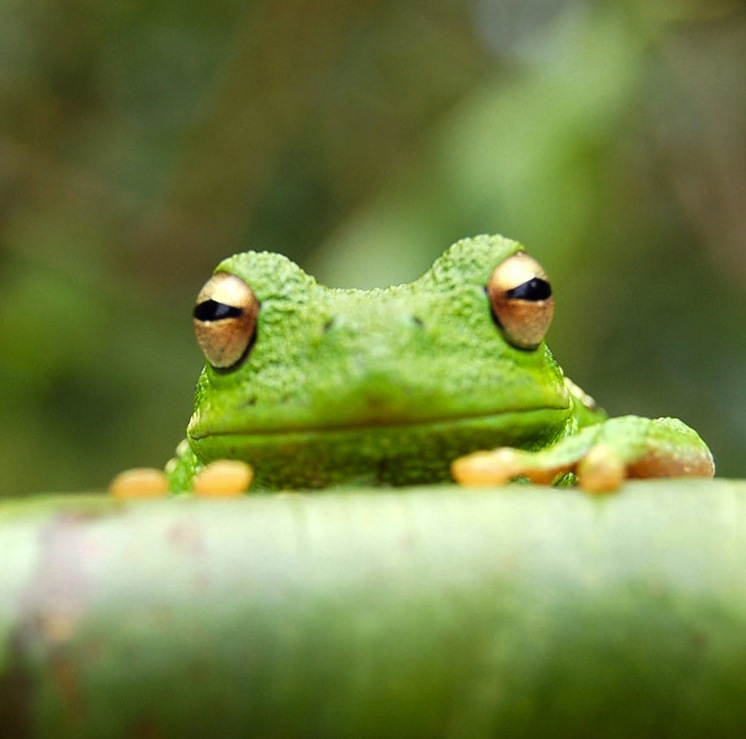
\includegraphics[width=\linewidth,height=7cm]{frog}
\captionof{figure}{This is a figure in the appendix}
\end{appendixbox}
\end{document}
